\chapter{Iteracion 6: Implementacion de un sistema gestionador para la placa de instrumentacion} % (fold)
\label{cha:iteracion_6}

\section{Introduccion} % (fold)
\label{sec:introduccion}

Para completar la prueba de campo, consideramos que es necesario testear el funcionamiento del sistema con algun embebido que tome la funcion de recibir los datos de telemetria y controlar la plataforma.

La plataforma diseñada, actualmente recibe, concentra, y distribuye datos de telemetria. Luego envia estos datos a otro sistema que realizara alguna accion en base a los datos recibidos. Esta iteracion se dedicará al desarrollo de un sistema de gestion simple, que implementa un servidor web con base de datos. La informacion de telemetria se guardara en esta base de datos, y sera posible accederla via internet. Ademas de esto, se proveera una interfaz grafica de usuario, que permita la configuracion tanto del sistema de gestion como de la plataforma.

El obejtivo principal es tener un sistema cuyas funciones incluyan el manejo de la plataforma de instrumentacion, pero que ademas, permita un uso mas general en lo que respecta al manejo de sistemas administradores de sensores y actuadores.

Este sistema fue construido con la ayuda del proyecto integrador de Gaston Lucero Berrini. Consiste en un sistema gestionador de dispositivos IoI. Parte del software de gestion del proyecto de Lucero, es un servidor web desarrollado en python, que es posible de embeber en una placa de desarrollo y actuar como el sistema gestionador al que se le envian los datos de telemetria. En esta iteracion, trabajaremos sobre este software, intentando adaptarlo al uso con nuestra plataforma, con el fin de cumplir con los objetivos de la iteracion.

% section introduccion (end)

\section{Requerimientos de la iteracion} % (fold)
\label{sec:requerimientos_de_la_iteracion}

\begin{itemize}
\item El sistema deberia estar implementado en una placa de desarrollo de manera que se pueda conectar a la placa de instrumentacion via comunicacion serial
\item Deberia estar en el mismo lugar fisico que la placa de alimentacion.
\item Deberia implementar un servidor web con una interfaz grafica de usuario. Esta interfaz deberia permitir:
\begin{itemize}
	\item La misma configuracion que se le permite a un usuario que esta conectado directamente a la placa de instrumentacion, via una interfaz web grafica con conexion a internet. 
	\item Enviar y recibir la respuesta de cualquier comando que pueda ser interpretado por la placa de instrumentacion
	\item Establecer intervalos de tiempo usando hora y fecha en los que se debe medir sobre algun canal, pudiendo elegir el modo y el intervalo del mismo.
\end{itemize}
\item Deberia guardar datos de mediciones e informacion sobre transacciones en general entre ambas placas en una base de datos local, accesible via la interfaz web grafica 
\item La conexion entre el sistema y el usuario (dispositivo del usuario: computadora con conexion a internet, smartphone) deberia ser via Wi-Fi o algun otro protocolo inalambrico
\end{itemize}


% section requerimientos_de_la_iteracion (end)


\section{Placa de desarrollo elegida para la implementacion} % (fold)
\label{sec:placa_de_desarrollo_elegida_para_la_implementacion}

Teniendo en cuenta los requerimientos, podemos listar una serie de requisitos que debe cumplir la placa de desarrollo que se seleccione:

\begin{itemize}
	\item Deberia poder albergar un sistema operativo basado en Linux o Unix
	\item Deberia permitir la conexion de un adaptador Wi-Fi USB
	\item Deberia tener interfaz serial UART
\end{itemize}

Por una cuestion de disponibilidad, decidimos implementar este sistema en una placa de desarrollo Raspberry Pi B+ (figura \ref{fig:raspberrypi}), embebida con un sistema operativo Raspbian (Debian para Raspberry). Esta placa de desarrollo cumple con todos los requisitos mencionados anteriormente, por lo que es posible cubrir todos los requerimientos del sistema de gestion.

\begin{figure}[h]
  \centering
  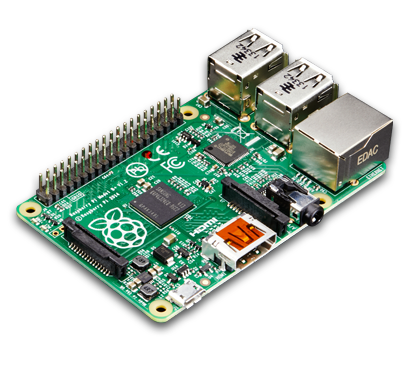
\includegraphics[width=0.80\textwidth, height = 7cm]{raspberrypi}
  \caption{Placa de desarrollo Raspberry Pi B+}\label{fig:raspberrypi}
\end{figure}
% section placa_de_desarrollo_elegida_para_la_implementacion (end)

\section{Diagramas de bloques} % (fold)
\label{sec:diagramas_de_bloques}

Como etapa inicial del desarrollo, procedemos a graficar diagramas de bloques que describen el diseño estatico del sistema.

\begin{figure}[h]
  \centering
  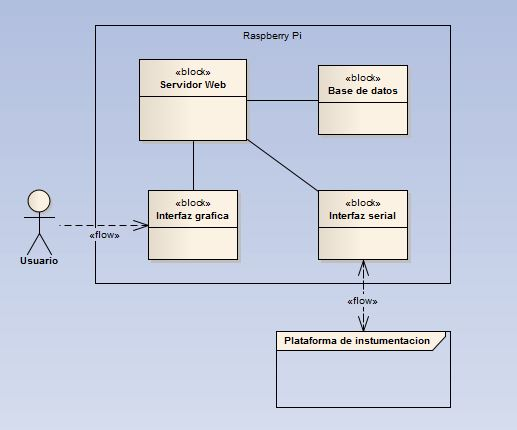
\includegraphics[width=0.80\textwidth, height = 7cm]{bloquessistemadegestion}
  \caption{Diagrama de bloques del sistema de gestion, implementado en una placa de desarrollo Raspberry Pi.}\label{fig:bloquessistemadegestion}
\end{figure}

\begin{figure}[h]
  \centering
  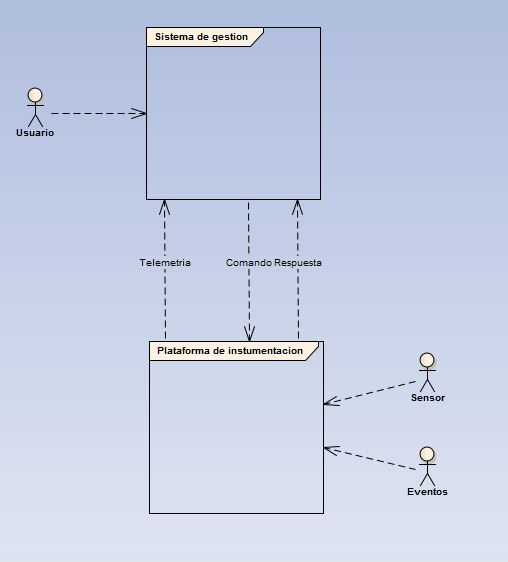
\includegraphics[width=0.80\textwidth, height = 7cm]{interaccionplataformaygestionador}
  \caption{Diagrama que ilustra la interaccion entre la plataforma de instrumentacion y el sistema gestionador}\label{fig:interaccionplataformaygestionador}
\end{figure}

La Figura \ref{fig:bloquessistemadegestion} muestra los distintos bloques del sistema de gestion y la figura \ref{fig:interaccionplataformaygestionador} ilustra la interaccion con la plataforma de instrumentacion. El sistema esta compuesto por cuatro bloques basicos:

\begin{itemize}
	\item Una interfaz grafica, que interactua con el usuario
	\item Una interfaz serial, que interactua con la plataforma de instrumentacion
	\item Un bloque que maneja el sistema de gestion de una base de datos MySQL, para guardar la informacion de telemetria junto con los metadatos
	\item Un Servidor Web, que ademas de proveer conexion a internet, maneja los bloques mencionados.
\end{itemize}


% section diagramas_de_bloques (end)

\section{Servidor web} % (fold)
\label{sec:servidor_web}


% section servidor_web (end)



\section{Base de datos} % (fold)
\label{sec:base_de_datos}

% section base_de_datos (end)

\section{Interfaz grafica de usuario} % (fold)
\label{sec:interfaz_grafica_de_usuario}



% section interfaz_grafica_de_usuario (end)


\section{Control del sensor de campo electrostatico} % (fold)
\label{it6:sub:control_desde_raspberry_pi}

En la iteracion 6, desarrollamos una adaptacion sobre la plataforma para poder utilizar un sensor de campo electrostatico en una prueba de campo. Los comandos de arranque y parada del sensor, y las mediciones de campo electrico, son controladas mediante comandos directos en la interfaz MML de la plataforma. \\

Con el desarrollo de esta iteracion, propusimos agregar las funcionalidades directamente ligadas al funcionamiento del sensor en la interfaz grafica del servidor web. De esta manera, el usuario tendria que unicamente presionar botones dentro de la interfaz grafica que se traducen en comandos que interpreta la plataforma, y de esta manera controlar el sensor. \\

A las funcionalidades disponibles del servidor, se le agregaron las posibilidades de:

\begin{itemize}
  \item Encender y apagar el motor
  \item Obtener mediciones instantaneas del sensor
  \item Configurar intervalos temporales de medicion. 
\end{itemize}

% subsection control_desde_raspberry_pi (end)


\section{Pruebas} % (fold)
\label{sec:pruebas}

% section pruebas (end)

\section{Resultados} % (fold)
\label{sec:resultados}

% section resultados (end)

% chapter iteracion_6 (end)